\documentclass[11pt, a4paper]{article}
\usepackage{amsmath, amssymb, graphicx, cmbright}
\newcommand{\dx}{\Delta x}
\newcommand{\dy}{\Delta y}
\newcommand{\Q}{\mathcal{Q}}
\title{Numerical Treatment of Differential Equations II \\ Exercise 1}
\date{January 15, 2009}
\begin{document}
\maketitle 

{\bf Topics:} Heat equation, finite volume method, conservation,
variable coefficients, boundary conditions.

{\bf Purpose:} This exercise builds on the basic course in numerical
treatment of differential equations. We will compute approximate
solutions to a time-dependent PDE on a 2D domain. Of particular
interest is the derivation of a basic finite volume method and how to
represent the discrete problem in a way that is practical for analysis
and implementation.

{\bf Instructions: } 
\begin{itemize}
\item Hand in a written report on the date indicated in the lecture
  and/or homepage. Report should contain answers to all questions
  stated and proper motivation for each, e.g. derivations. Submit code
  via e-mail.
\item If you work alone, choose either to answer section
  \ref{sec:varcoeff} (variable coefficients) or section \ref{sec:bc}
  (boundary conditions). If you work in pairs, you must answer both.
\end{itemize}

\section{Heat equation}
A classical example of an parabolic PDE is the heat equation on a square. Let
$q(x,y,t)$ denote temperature. Then,
\begin{align}
  q_t &= \nabla \cdot (\nabla q) + S, \quad (x,y) \in [0 \,\, 1] \times [0 \,\, 1], t \geq 0 \label{pde}\\
  q(x,y,0) &= 0\\
  \hat{n}\cdot \nabla q &= 0, \quad (x,y) \text{ on boundary} \label{bc}
\end{align}
We have a heat source at the point, (1/2,1/2),
\begin{align*}
  S(x,y,t) & = \delta(x-1/2) \delta(y-1/2) g(t)\\
  g(t) & =
  \begin{cases}
    2\quad \text{ if } 0 \leq t \leq 1/4 \\
    0\quad \text{ otherwise}.
  \end{cases}
\end{align*}
The boundary conditions \eqref{bc} state that there
is no heat flux across boundaries. Physically, we have a plate that is
insulated from its surroundings and initially at zero temperature. It
is heated at a point for 0.25 seconds and then the source is turned
off.
\subsection{Analytical preamble} \label{sub:ap}
\begin{enumerate}
\item Determine $\tilde{Q}(t) = \int_0^1 \int_0^1 q(x,y,t) dx dy$ as a
  function of $t$.
\end{enumerate}
\section{Discretization and implementation}
Let $Q_{ij}$ denote the cell average of $q$ over cell $(i,j)$ (see
Figure \ref{fig:fv_grid}) and introduce cell sizes $\dx$ and $\dy$
such that $m\dx = n\dy = 1$.
\begin{figure}
  \centering
  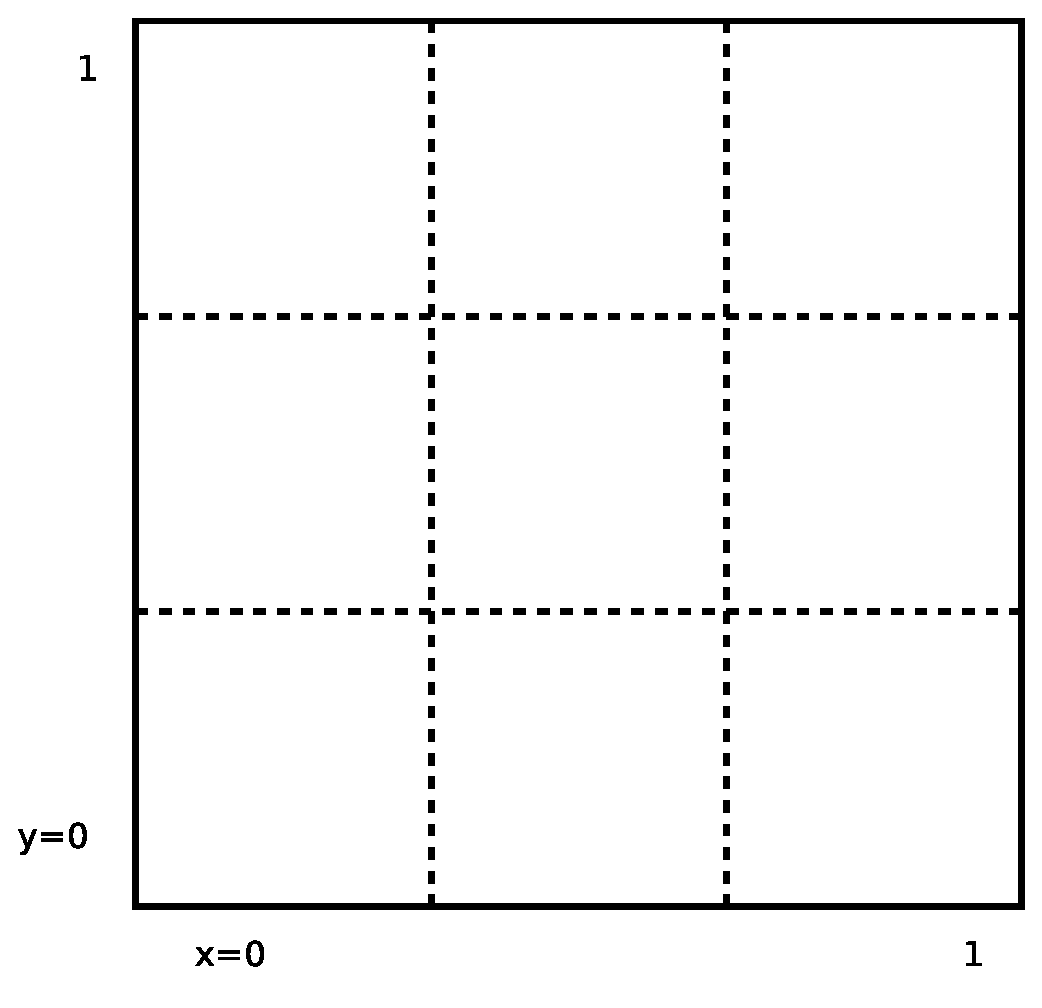
\includegraphics[scale=0.4]{fig/grid1}
  \caption{Finite volume grid}
  \label{fig:fv_grid}
\end{figure}
\begin{enumerate}
\item Derive a conservative finite volume method for the spatial part
  of \eqref{pde} by integrating and forming cell averages. Take care
  that the source term gets included correctly. Show that you obtain
  an expression of the form
  \begin{align*}
    \frac{d}{dt} Q_{ij} = \Delta_5 Q_{ij} + S_{ij}, \quad (i,j) \text{
      interior indices}
  \end{align*}
  where $\Delta_5$ is the five-point Laplacian stencil familiar from
  finite difference methods. What stencils do you get at the
  boundaries? 
\item Integrate in time using the first order implicit Euler
  scheme. Why is this more appropriate than explicit? \emph{Hint:}
  time-step restriction. State the fully discrete problem.
\item Let $\Q$ be an $m\times n$ array that contains the $Q_{ij}$
  values. The Laplacian can be expressed as\footnote{cf. supplementary
    material from Demmel}
  \begin{align*}
    \Delta_5\Q = \Q T_x + T_y \Q 
  \end{align*}
  where $T$ represents the Laplacian difference operator in 1D for
  each dimension respectively. Why is this convenient? \emph{Hint:}
  Boundary conditions. Use this idea to state the fully discrete
  problem in matrix form. 

  Prove that the finite volume scheme is \emph{exactly} conservative.
\item Implement the finite volume method, e.g. in MATLAB. 

  A linear system has to be solved in each time-step. Due to the
  boundary conditions, this matrix has a block diagonal structure (it
  is {\bf not} simply diagonal). Constructing it can be fairly hard in
  a Matlab program, and possibly \emph{very} computationally
  inefficient (see example in ``Notes on Efficient Matlab
  Programming'').

  A good option is to use Kronecker products
  \footnote{cf. http://en.wikipedia.org/wiki/Kronecker\_product } to
  construct this difference matrix. The corresponding function is
  called \verb|kron| in Matlab. It is highly recommended to use the
  function \verb|reshape| to rearrange a $m\times n$ array into a
  $mn\times 1$ column vector and vice versa.

  When you think the program works, compare your solutions to the
  reference plots posted on the web page.

  You are strongly encouraged to write an efficient program -- one that
  can handle fine resolutions in reasonable time. Take care to make
  the code clean and readable. On an average workstation the solver
  may be able to handle $m = n = 800$ or more without much trouble
  (aside from plotting such a large data set). To get this efficiency,
  try to move as much work as possible out of the time loop. Use the
  profiler in Matlab! \emph{Hint:} Is the matrix in the linear system
  constant in time? Consider LU-factorizing (using the function
  \verb|lu| in Matlab).
\end{enumerate}

\section{Numerical results} \label{sec:numres}
In your report, please include the following computational results:
\begin{description}
\item[Solution plots] for some time levels before and after $t=1/4$.
\item[Convergence] Choose a point $(x_0,y_0)$ and compile a table which
  shows that the error behaves like $\mathcal{O}(\Delta t^p) +
  \mathcal{O}(h^r)$, where $h = \dx = \dy$. Determine $p$ and
  $r$. What would one anticipate from theory? Why is it a bad idea to
  look at the error in $\infty-$ or $L_2$-norm?
\item[Numerical conservation] Demonstrate that the method is
  numerically conservative by looking at $\int q dx dy =
  \dx\dy\sum_{ij} Q_{ij}$ for all $t$. Compare it to the expression
  computed in Section \ref{sub:ap}. Conservation in ``eye norm'' is
  not enough!
\end{description}
\section{Refinements}
Now we move on to slightly more advanced problems. The framework
developed thus far in this lab should be very helpful when you tackle
these problems. Do {\bf not} proceed with these tasks until the
program above works as expected!
\subsection{Variable coefficients} \label{sec:varcoeff}
Consider
\begin{align}
  q_t = a(y) q_{xx} + b(x) q_{yy} + S
\end{align}
instead of the PDE \eqref{pde}. Choose $a(y)$ and $b(x)$ as smooth and
positive functions.
\begin{enumerate}
\item Formulate the fully discrete problem for the variable
  coefficient case, preferably in the Kronecker notation. \emph{Hint:}
  Multiplication from the left with a diagonal matrix scale each row
  of a matrix. How do you scale the columns?
\item Implement the variable coefficient problem. With the Kronecker
  product construction, this should be fairly simple.

  Present convergence and conservation results as in section \ref{sec:numres}
\end{enumerate}
\subsection{Boundary conditions} \label{sec:bc}
Change the boundary conditions \eqref{bc} to
\begin{align*}
  q(0,y,t) &= \frac{1}{\pi}\sin(\pi y)\\
  q(1,y,t) &= \frac{1}{3\pi}\sin(3 \pi y)+1\\
  q_y(x,0,t) &= -1\\
  q_y(x,1,t) &= -1
\end{align*}
You may choose a different set of boundary conditions if you want to,
as long as you include at leas one non-homogeneous Neuman and Dirichlet
condition. 
\begin{enumerate}
\item Implement this new boundary condition. 
 
  The approach is as follows: Construct 1D difference matrices for
  each dimension and make sure they express the right boundary
  conditions. Then assemble the 2D difference matrix from the 1D
  matrices using Kronecker products. \emph{Hint:} In the matrix form
  of of the fully discrete problem only one of the $T$ operators needs
  to change (in the case of the suggested new BC).

  There are different options for how to enforce Dirichlet BCs in a
  finite volume method. For the suggested boundary conditions, you may
  choose the grid given in Figure \ref{fig:grid_2}.

  Present convergence results as in section \ref{sec:numres} and
  discuss conservation in the context of non-homogenous boundary
  conditions.
\end{enumerate}
\begin{figure}
  \centering
  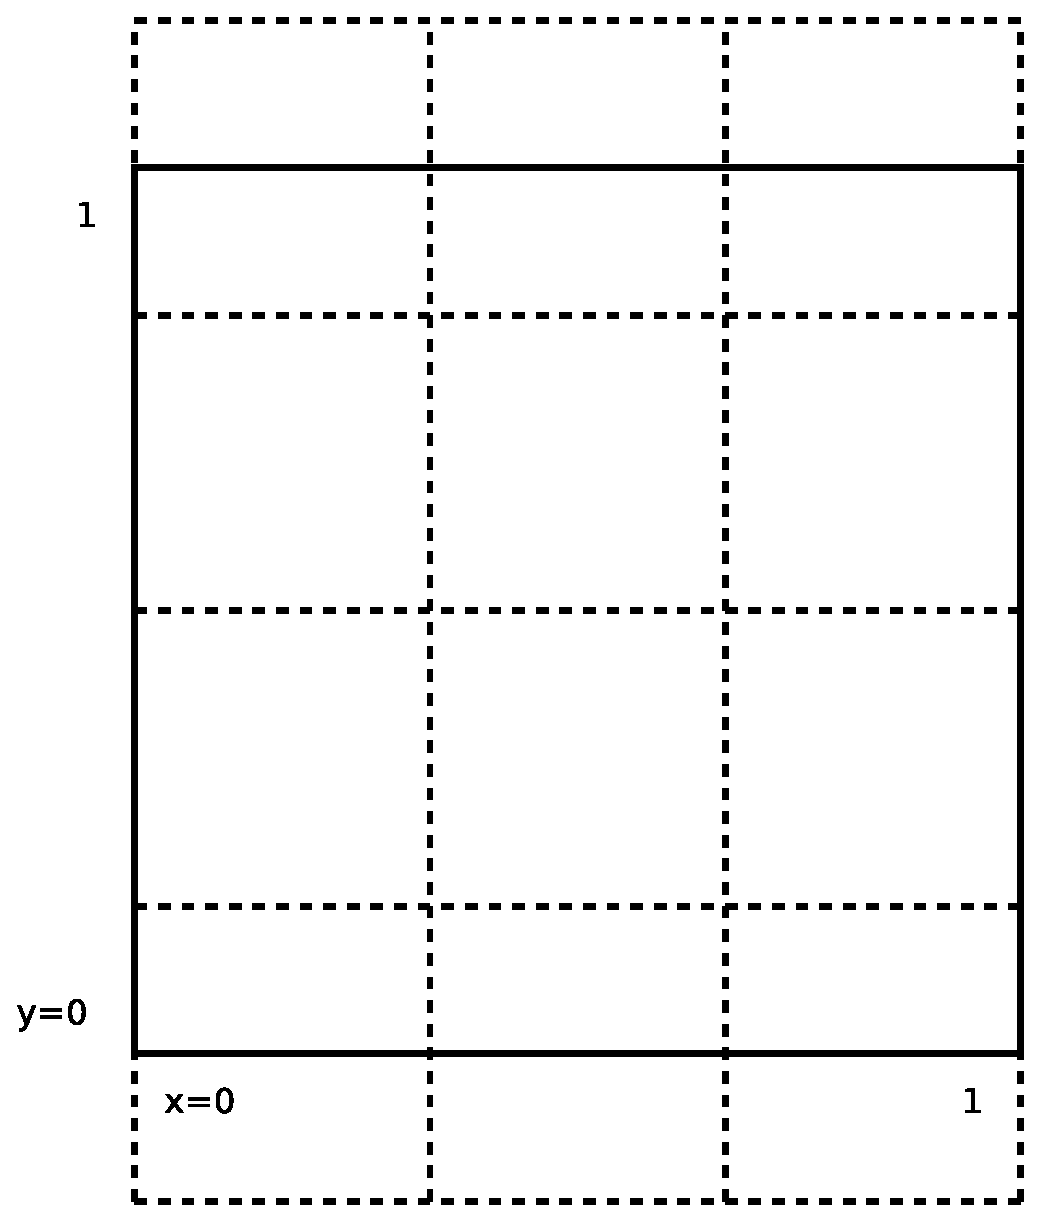
\includegraphics[scale=0.4]{fig/grid2}
  \caption{Staggered finite volume grid}
  \label{fig:grid_2}
\end{figure}

\end{document}
